%% Los margenes, tipo de hoja y estilo BOOK
\documentclass[a4paper,11pt,twoside,openright,titlepage]{book}
\usepackage[a4paper,left=1in,right=1in,top=0.6in]{geometry}

\usepackage[T1]{fontenc}    %Ineterprete de t�ldes
%\usepackage[Latin1]{inputenc}
\usepackage{amsmath,amssymb}    %Paquete de entornos matematicos

\usepackage{natbib}

\usepackage[english,spanish]{babel}
\selectlanguage{spanish} 
\usepackage{graphicx}
\usepackage{psfrag}
\usepackage{quotchap}
\usepackage{epsfig}
\usepackage[all]{xy}

\usepackage{epsfig}
\usepackage{makeidx}
\usepackage{ifthen}
\usepackage{multicolpar}    %Para poner texto en columnas en plan articulo intercalado con texto normal
\usepackage{multicol,multirow}

\usepackage{url}        %Para direcciones web
\usepackage{marvosym}   %Para imprimir el simbolo de \EUR euro
%\usepackage{eurosym}   %Para imprimir el simbolo de \euro euro
\usepackage{fancybox}   %Para tablas con bordes redondeados


\usepackage{listings} 	%Para importar c�digo
\usepackage{minted}		%Para que se vea bonito el c�digo
\usepackage{todonotes}	%Para marcar lo que queda por hacer
\usepackage{nameref}	%Para referenciar la secci�n actual
\usepackage{csquotes}	%Para texto entre comillas
\usepackage[hidelinks]{hyperref} 	%Para hacer las tablas de contenido clickables
\usepackage{caption}
%\usepackage[all]{hypcap}

\makeatletter
\newcommand*{\currentname}{\@currentlabelname}
\makeatother

%% Modificaci�n de la plantilla para adaptarla a los requisitos de PFC
\usepackage{fancyhdr}
\pagestyle{fancy}
%%% Cabeceras y pies de p�gina
\fancyhead[CE,CO]{\emph{\titulo}}
\fancyhead[LE,LO,RE,RO]{}
\fancyfoot[LE,RO]{\thepage}
\fancyfoot[CE,CO]{\leftmark}

\renewcommand{\footrulewidth}{.6pt}


%Definiciones de funciones para los titulos
\newlength\salto
\setlength{\salto}{3.5ex plus 1ex minus .2ex}

\newlength\resalto
\setlength{\resalto}{2.3ex plus.2ex}

\newcommand{\lsection}[1]
                {\section{#1}
                \vskip-.9\resalto   %%%% Aqu� reculo el posible salto por defecto de \section
                \hrule
                \vskip+.9\salto}  %%%% vuelvo ha realizar el salto (puedes poner otra vez el 90%)


%Para im�genes de entornos est�ticos \captionFigure{Texto Caption}{Texto Label}
\newcommand{\captionFigure}[2]{
    \refstepcounter{figure}
    \centerline{Figura \thefigure: #1 \label{#2}}
    \addcontentsline{lof}{section}{\thefigure.\ #1\label{#2}}
}

%Para im�genes de entornos est�ticos \NOcaptionFigure{Texto Caption}{Texto Label} "No escribe el caption"
\newcommand{\NOcaptionFigure}[2]{
    \refstepcounter{figure}
    \addcontentsline{lof}{figure}{\thefigure.\ #1\label{#2}}
}


%% Datos del PFC
\newcommand{\titulo}{Google Cardboard Robotic Avatar}
\newcommand{\autor}{Autor: Borja Mauricio Fourquet Maldonado}
\newcommand{\director}{Nombre Apellido1 Apellido2}
\newcommand{\tutor}{Tutor: Francisco Saiz L�pez}
\newcommand{\ponente}{Ponente: Nombre Apellido1 Apellido2}
\newcommand{\vocal}{Nombre Apellido1 Apellido2}
\newcommand{\vocalsup}{Nombre Apellido1 Apellido2}
\newcommand{\presidente}{Nombre Apellido1 Apellido2}
\newcommand{\presidentesup}{Nombre Apellido1 Apellido2}
\newcommand{\fecha}{Junio 2016}
\newcommand{\carrera}{Grado en Ingenier�a Inform�tica}
\newcommand{\producto}{\textit{Google Cardboard Robotic Avatar} }

\begin{document}
\setlength{\baselineskip}{18pt}  %% Espacio interlinea
\setlength{\parskip}{6pt plus 1pt minus 1pt} %% Espacio interp�rrafo

\begin{titlepage}

\begin{center}

\vspace*{2cm}

\LARGE \textsc{Universidad Aut�noma de Madrid}\\

\vspace{.2cm}

\large \textsc{Escuela polit�cnica superior}\\

\vspace{.2cm}

\begin{figure}[h]
    \begin{center}
        \begin{minipage}[c]{0.495\linewidth}
            \rightline{\epsfig{figure=images/logo_eps.eps,width=0.5\linewidth}}
        \end{minipage}
        \begin{minipage}[c]{0.495\linewidth}
            \leftline{\epsfig{figure=images/logo_uam.eps,width=0.5\linewidth}}
        \end{minipage}
    \end{center}
    \label{fig:Escudos}
\end{figure}

\Huge \carrera\\

\vspace{1cm}

\Huge \textsc{Trabajo Fin de Grado}\\

\vspace{1.5cm}

\Huge \MakeUppercase{\textbf{\titulo}}

\vspace{3cm}


\Large \autor\\
\Large \tutor\\


\vspace{0.5cm}

\Large \fecha

\end{center}

\end{titlepage}

\normalsize


\newpage \thispagestyle{empty} % P�gina vac�a


\frontmatter %Define el cuerpo inicial del libro en numeraci�n con letras romanas

\chapter*{}

\vspace*{0.2cm}

\begin{center}

\Huge \MakeUppercase{\textbf{\titulo}}

\vspace{7cm}

\Large \autor \\
\Large \tutor \\


\vspace{5cm}


Escuela Polit�cnica Superior \\
Universidad Aut�noma de Madrid \\
\fecha

\end{center}

\normalsize

\newpage \thispagestyle{empty} % P�gina vac�a


\chapter*{Resumen}

\section*{Resumen}
\todo[inline]{ \currentname}
\section*{Palabras Clave}
\todo[inline]{ \currentname}
\newpage

%-------------------------------------------------------------------------------------------------------------------------------------
\section*{Abstract}
\todo[inline]{ \currentname}
\section*{Key words}
\todo[inline]{ \currentname}

\chapter*{Agradecimientos}

A mi tutor en este proyecto, Francisco Saiz, por acompa�arme en esta aventura hasta el final.

A los profesores que, con su inter�s por el progreso de los alumnos y su sabidur�a, me han motivado a seguir aprendiendo y super�ndome personalmente.

A los profesores que, con su falta de inter�s, indirectamente me han ense�ado a apa��rmelas y a aprender por mi cuenta.

A mi familia, que se preguntaban qu� hac�a desde que amanec�a hasta que se pon�a el sol en la escuela y que me han apoyado cuando la carrera se hac�a cuesta arriba.

\listoftodos

\tableofcontents

\newpage \thispagestyle{empty} % P�gina vac�a

\addcontentsline{toc}{chapter}{�ndice de Figuras}    %Para que aparezca en el �ndice
\renewcommand{\listfigurename}{�ndice de Figuras} 
\listoffigures

\newpage \thispagestyle{empty} % P�gina vac�a

\addcontentsline{toc}{chapter}{�ndice de Tablas}    %Para que aparezca en el �ndice
\renewcommand{\listtablename}{�ndice de Tablas} 
\listoftables

\newpage \thispagestyle{empty} % P�gina vac�a

\mainmatter %Define el cuerpo principal del libro numeraci�n normal.

% \input{preambulo}

\chapter{Introducci�n} 
\label{chap:intro}

\vspace{-0.2cm}

\textit{A little imagination, the right tools, and you can have a virtual world at your fingertips...}

\lsection{Motivaci�n del proyecto}

Mi motivaci�n personal a la hora de embarcarme en este proyecto es la de crear un sistema inform�tico heterog�neo, investigando as� campos como la programaci�n para dispositivos m�viles (en este caso, para Android) y las redes multimedia.

Por otra parte, mi inter�s por la realidad virtual, que tanto est� creciendo en cuesti�n de meses, me lleva a integrarla en este proyecto.

Por �ltimo, mi experiencia en las pr�cticas de empresa que realic� en el proyecto de emprendimiento The Haptic Eye \cite{link:the_haptic_eye} me animaron a llevar a cabo otro proyecto innovador, en tiempo real y que re�na tecnolog�as punteras en el estado del arte.


\lsection{Objetivos y enfoque}

% Esto quiz�s en el abstract mejor
%A modo de s�ntesis, el objetivo inicial es desarrollar un sistema que proporcionara visi�n remota al
%usuario mediante de un smartphone conectado, a trav�s de Internet, con un robot con dos c�maras
%como si este �ltimo se tratase de un avatar.
%
%El sistema consta, principalmente, de dos partes:
%\begin{enumerate}  
%\item Un Google Cardboard y un tel�fono m�vil con Android desde el que ejecutar la
%aplicaci�n. �sta estar� desarrollada utilizando la API de Google Cardboard [2]. En vez de
%renderizar gr�ficos en 3D (Figura~\ref{fig:cardboard_3d}), simplemente se reproducir�n en tiempo real simult�neamente
%dos v�deos (uno para cada ojo).


%\item Un peque�o robot con las siguientes caracter�sticas:
%\end{enumerate}
%\begin{itemize}
%\item Dos videoc�maras.
%\item Una estructura donde alojar estas dos c�maras.
%\item Un motor que haga girar esta estructura sobre el eje vertical (Figura~\ref{fig:movimiento_cabeza})
%\item Conectividad con la aplicaci�n a trav�s de Internet.
%\end{itemize}


\begin{itemize}
	
	\item Investigar los distintos protocolos e implementaciones de transmisi�n de v�deo en tiempo real a trav�s de la red  para encontrar el m�s id�neo para este proyecto.
	\item Aprender los fundamentos de la programaci�n de aplicaciones para dispositivos m�viles, as� como familiarizarme con el uso del IDE Android Studio.
	\item Asimilar las bases de la realidad virtual y, concretamente, de las aplicaciones para las gafas de VR \textit{Google Cardboard} o similares (figura \ref{fig:googlecardboard}).
	\item Dise�ar el sistema del producto, tanto \textit{front-end} como \textit{back-end}, teniendo en cuenta las caracter�sticas distribuidas y en tiempo real del software para crear un prototipo, a modo de prueba de concepto (POC), con las funcionalidades b�sicas.
	\item Redactar unas conclusiones del proyecto que sirvan de gu�a a toda aquella persona que se aventure en un proyecto similar y enumerar las posibles mejoras futuras a partir de las facilidades e impedimentos que se han dado en el desarrollo de este prototipo y teniendo en mente el estado actual de las tecnolog�as implicadas, as� como las perspectivas de que �stas crezcan y mejoren en el futuro inmediato.
	
\end{itemize}



\begin{figure}[h]
	\centerline{
		\mbox{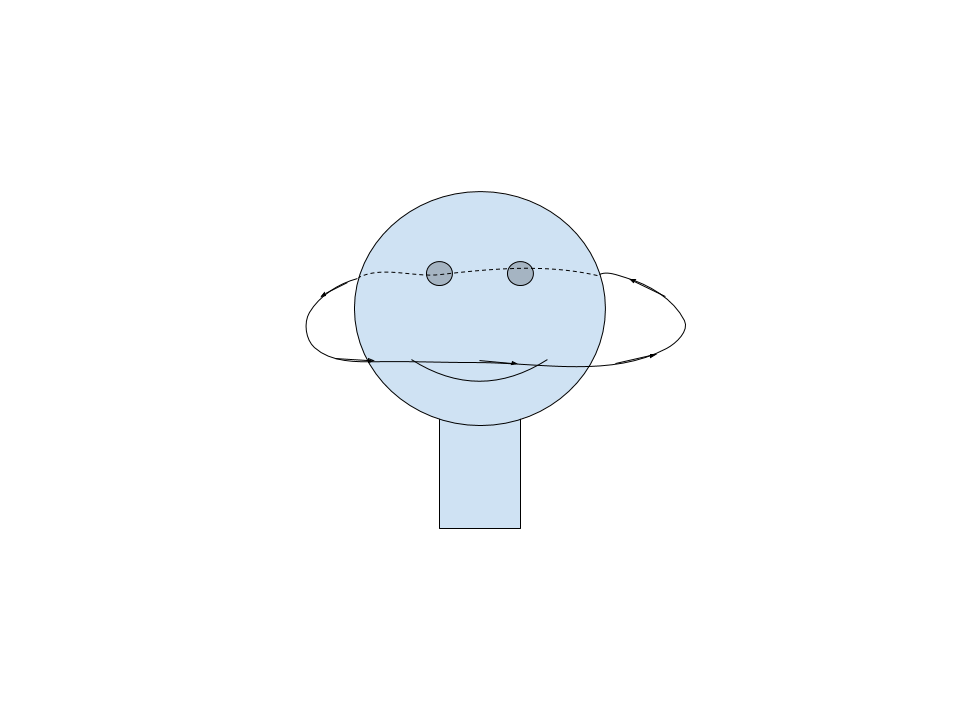
\includegraphics[width=3.00in]{images/movimiento_cabeza.png}}
	}
	\caption{\textbf{Movimiento de la cabeza} alrededor del eje vertical}
	\label{fig:movimiento_cabeza}
\end{figure}

\begin{figure}[h]
	\centerline{
		\mbox{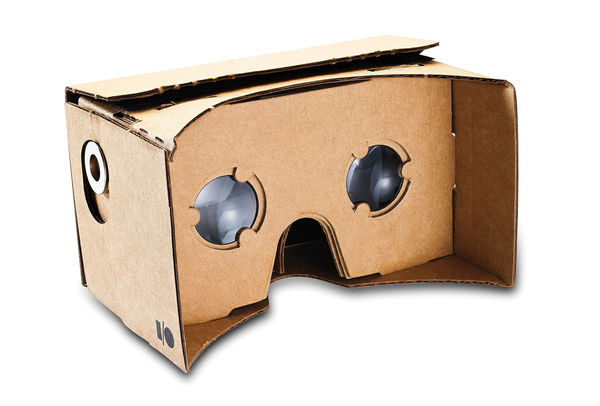
\includegraphics[width=3.00in]{images/googlecardboard.jpg}}
	}
	\caption{\textbf{Google Carbdoard}: las gafas de realidad virtual a partir de unas lentes, cart�n y un smartphone}
	\label{fig:googlecardboard}
\end{figure}

%La aplicaci�n recibir� como entrada dos streams correspondientes a las c�maras de la
%segunda parte y la posici�n en la que esta parte se encuentra (aunque en la pr�ctica esto �ltimo
%quiz�s no haga falta). Como salida, enviar� la posici�n en la que se encuentra la cabeza del usuario
%como comandos que el subsistema 2 procesar� y convertir� en instrucciones para los motores que
%mueven su estructura.


\lsection{Metodolog�a y plan de trabajo}

En este apartado se enumeran las herramientas utilizadas para llevar a cabo este proyecto.

\subsection{Recursos}

Estos son los recursos f�sicos m�s significativos utilizados en este proyecto.

\begin{itemize}
	\item PC con procesador \textbf{Intel Core i7} 4790K @ 4.0GHz
	\item \textbf{Arduino UNO}
	\item \textbf{Servomotor} a 3.3V
	\item \textbf{Videoc�maras USB} corrientes (\textit{webcams}) x 2
\end{itemize}


\subsection{Producci�n}

La producci�n de todo el software se ha llevado a cabo en el PC de sobremesa anteriormente mencionado.

\begin{itemize}

	\item \textbf{Ubuntu 14.04}: popular sistema operativo basado en Debian.
	\item Repositorio en \textbf{BitBucket} con git (\url{https://bitbucket.org/})
	\item \textbf{Android Studio} para el cliente Android del sistema
	\item \textbf{Eclipse Mars.2} para el cliente con JavaCV
	\item \textbf{Sublime Text 3} para editar archivos Bash, Makefiles y c�digo Python.
	\item \textbf{Arduino IDE} para el c�digo de la placa Arduino 

\end{itemize}


\subsection{Despliegue}

El despliegue de los servidores se lleva a cabo mediante la terminal de Linux

\begin{itemize}
	\item \textbf{Ubuntu 14.04}
	\item \textbf{Makefile}
	\item \textbf{Bash}
	\item \textbf{cvlc} (VLC para la terminal de Linux)
\end{itemize}


\subsection{Documentaci�n}

La documentaci�n se ha elaborado utilizando las siguientes herramientas:

\begin{itemize}
	\item \textbf{TeXstudio}: editor de documentos LaTeX.
	\item \textbf{Creately}: aplicaci�n web para el dise�o de diagramas que puede ser utilzada en \url{http://creately.com/} 
	\item \textbf{README.md} de BitBucket. Markdown (.md) es un lenguaje de marcas, mucho m�s simple que HTML, orientado a documentar repositorios.
\end{itemize}


\newpage \thispagestyle{empty} % P�gina vac�a 

\chapter{Estado del arte}
\label{chap:estadodelarte}
 
\lsection{Introducci�n}
\todo[inline]{Estado del arte: \currentname}
La realidad virtual es un concepto que existe desde hace d�cadas, aunque durante gran
parte de este tiempo se ha visto como mera ciencia ficci�n. Actualmente, ya existen dispositivos dise�ados espec�ficamente para que el usuario pueda visualizar mundos virtuales en 3D. 

En primavera de 2016 se concentran las fechas en las que numerosas empresas prometieron
comercializar productos con esta funcionalidad, como son Oculus Rift, HTC Vive y PlayStation VR entre otros. 

Por otra parte, la realidad aumentada combina en tiempo real la visi�n del entorno f�sico
con elementos virtuales que a�aden informaci�n a lo que uno podr�a ver simplemente con sus ojos. Microsoft Hololens llegar� al mercado tambi�n en la primera mitad del a�o 2016.
El producto descrito a continuaci�n no se podr�a clasificar como ninguno de estos dos
anteriores, aunque s� que es cierto que est� fuertemente ligado a estos dos conceptos.
En septiembre de 2015, Snapchat incorpora la realidad aumentada a su aplicaci�n, pudiendo personalizar fotograf�as y v�deos en tiempo real con distinto contenido basado en el reconocimiento facial.

%\lsection{Definici�n.} \label{sec:definicion}

\lsection{Historia, nacimiento y evoluci�n.} \label{sec:historia}
\todo[inline]{Estado del arte: \currentname}


\lsection{Estado actual}  \label{sec:estadoactual}
\todo[inline]{Estado del arte: \currentname}

\lsection{Conceptos previos} \label{sec:conceptosprevios}
\todo[inline]{Estado del arte: \currentname}
\newpage \thispagestyle{empty} % P�gina vac�a 

\chapter{An�lisis, arquitectura y dise�o del sistema}
\label{chap:sistemadesarrollado}

\lsection{An�lisis}
\subsection{Descripci�n del producto}
\producto es un producto que permite al usuario ver a trav�s de los ojos de un avatar. Esto se consigue gracias a unas gafas de realidad virtual *REFERENCIA FIGURA* conectadas a trav�s Internet a un robot con dos c�maras por ojos. Los movimientos de la cabeza del usuario ser�n tambi�n transmitidos a trav�s de la red hasta llegar al robot, que ejecuta un programa que recibe estos datos y actualiza la orientaci�n de las c�maras en tiempo real para dar la sensaci�n al usuario final de estar en otro cuerpo.

\todo[inline]{Referencia a gafas de VR: \currentname}
\subsection{Viabilidad}
1

\todo[inline]{An�lisis: \currentname}

\subsection{Objetivos y funcionalidad}

El objetivo principal del proyecto es el de desarrollar un sistema con los siguientes tres elementos:
\begin{enumerate}
\item Dos \textbf{servidores de v�deo} que reciban como entrada un dispositivo cada uno (en este caso, una c�mara por servidor) y como salida ofrezcan un \textit{stream} multimedia.
\item Un \textbf{servidor de control} que reciba el posicionamiento del dispositivo de realidad virtual y asigne un valor anal�gico a los actuadores a partir de las coordenadas, que ser�n los motores sobre los que se encuentra la estructura en la que reposen las c�maras.
\item Una \textbf{aplicaci�n para dispositivo smartphone} que establezca la conexi�n con los servidores. Recibir� como entrada dos \textit{streams} de v�deo (uno por cada ojo) y como salida enviar� la rotaci�n respecto de los tres ejes dimensionales.
\end{enumerate}

\begin{figure}[h]
	\centerline{
		\mbox{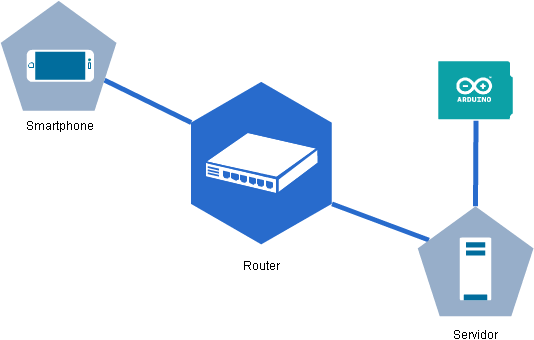
\includegraphics[width=4.00in]{images/diagrama_red_fisico.png}}
	}
	\caption{\textbf{Diagrama conceptual de la red del sistema}}
	\label{fig:diagrama_red}
\end{figure}


S�lo existe un tipo de usuario de la aplicaci�n y, en un principio, su interacci�n se limitar� a la siguiente:

\begin{itemize}
	\item Alterar la posici�n f�sica de las gafas de realidad virtual girando la cabeza.
	\item Modificar la direcci�n IP y los puertos de sendos servidores a trav�s de la pantalla t�ctil del smartphone.
\end{itemize}




El sistema no deber�a necesitar ning�n tipo de persistencia. Las conexiones se realizar�an en modo \textit{stateless}, lo que quiere decir el cliente se conecta y desconecta de los servidores arbitrariamente sin que deban almacenarse datos de sesi�n algunos.

\subsection{Requisitos}
\begin{enumerate}
	\item Las im�genes se transmiten y se muestran con baja latencia.
	\item Los distintos objetos comunes en las dos im�genes se pueden apreciar en tres dimensiones.
	\item Los consecutivos movimientos de la cabeza son transmitidos secuencialmente y con baja latencia.	
	\item El usuario puede modificar la direcci�n IP de cada servidor.
	\item El usuario puede modificar el puerto de cada servidor.
\end{enumerate}
\subsection{Tama�o y rendimiento}
Esta arquitectura del software est� orientada a permitir exclusivamente una conexi�n simult�nea. Al tratarse de una aplicaci�n en tiempo real, m�s conexiones podr�an congestionar el tr�fico en la red y saturar los recursos de los servidores. Adem�s, la rotaci�n de los motores s�lo deber�a controlarse desde un solo cliente.


\begin{figure}[H]
	\centerline{
		\mbox{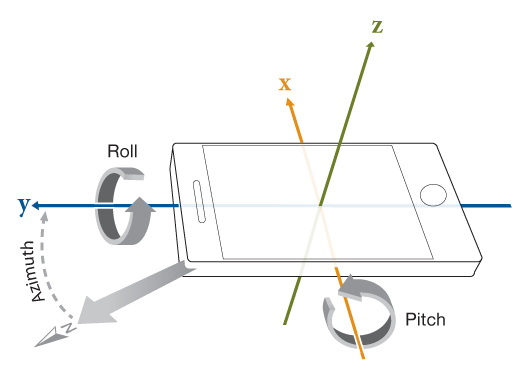
\includegraphics[width=4.00in]{images/coordinates.jpg}}
	}
	\caption{\textbf{Coordenadas polares}. Azimuth ($\Psi$), Pitch ($\Phi$), Roll ($\theta$)}
	\label{fig:coordenadas_polares}
\end{figure}


\lsection{Arquitectura}

\subsection{Vista est�tica}

El cliente es el componente central de este sistema heterog�neo. �ste est� compuesto a su vez de otros tres componentes que se ejecutan como hilos independientes en la app. Uno de ellos env�a peri�dicamente la orientaci�n del dispositivo al servidor de control en datagramas a trav�s del protocolo de transporte UDP. Los otros dos reciben un stream de v�deo cada uno, procedentes de los servidores de v�deo a trav�s del protocolo de aplicaci�n RTSP. El servidor de control est� conectado a su vez con el Arduino por medio de USB, al igual que las c�maras est�n conectadas a la m�quina en la que se ejecutan los servidores de v�deos tambi�n por USB. Estas relaciones entre los componentes se pueden visualizar en la figura~\ref{fig:diagrama_componentes}

\begin{figure}[H]
	\centerline{
		\mbox{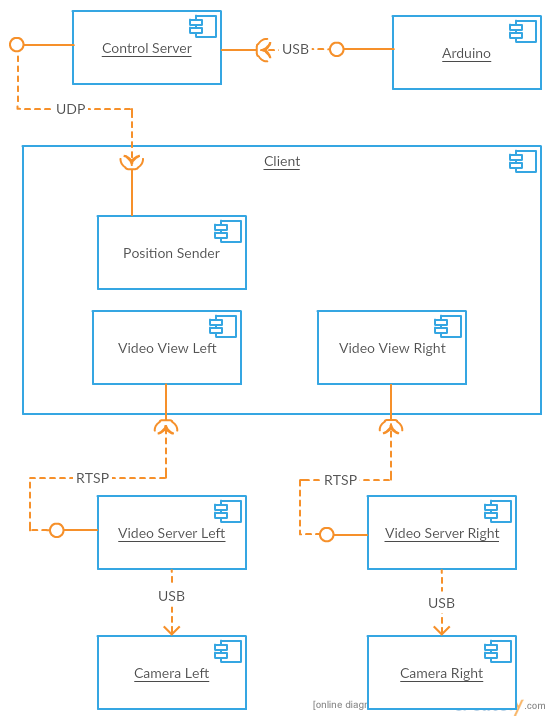
\includegraphics[width=4.00in]{images/diagrama_componentes.png}}
	}
	\caption{\textbf{Diagrama de componentes del sistema}. Se pueden apreciar los distintos componentes, las interfaces que ofrecen y requieren y el protocolo que utilizan para comunicarse entre s�.}
	\label{fig:diagrama_componentes}
\end{figure}



\subsection{Vista funcional} % La visi�n funcional: describe qu� hace cada componente.

Aqu� ir�a una explicaci�n detallada de la funcionalidad de cada componente por separado

\subsubsection{Servidor de v�deo}
\todo[inline]{Vista funcional: \currentname}
\subsubsection{Servidor de control}
\todo[inline]{Vista funcional: \currentname}
\subsubsection{Cliente m�vil}
\todo[inline]{Vista funcional: \currentname}

\subsection{Vista din�mica} % La visi�n din�mica: describe c�mo se comportan los componentes a lo largo del tiempo y como interact�an entre s�.
\todo[inline]{\currentname}
Aqu� se muestra c�mo evoluciona el sistema con el tiempo y dados ciertos eventos.

\lsection{Dise�o}

\subsection{Servidor de v�deo}
\todo[inline]{Dise�o: \currentname}
\subsection{Servidor de control}
\todo[inline]{Dise�o: \currentname}

\begin{figure}[H]
	\centerline{
		\mbox{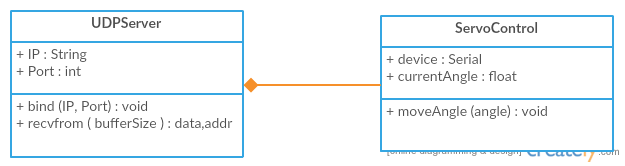
\includegraphics[width=4.00in]{images/diagrama_clases_servidor_control.png}}
	}
	\caption{Diagrama de clases del servidor de control}
	\label{fig:diagrama_clases_servidor_control}
\end{figure}

\subsection{Cliente m�vil}
\todo[inline]{Dise�o: \currentname}
\begin{figure}[H]
	\centerline{
		\mbox{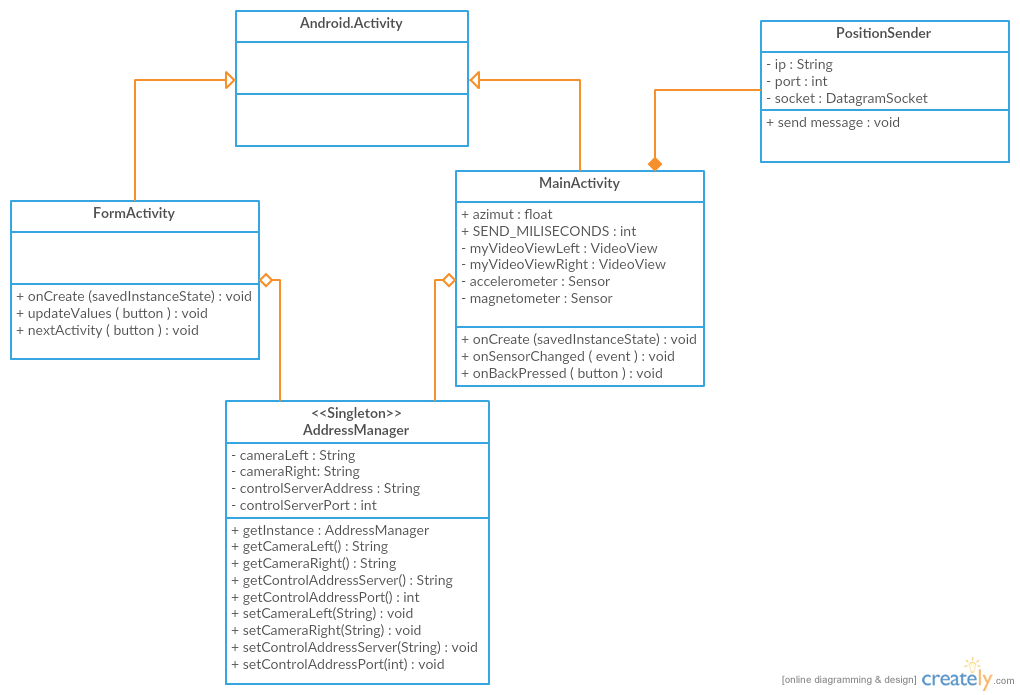
\includegraphics[width=7.00in]{images/diagrama_clases_app.png}}
	}
	\caption{Diagrama de clases de la aplicaci�n para Android}
	\label{fig:diagrama_clases_app}
\end{figure}

\begin{figure}[H]
	\centerline{
		\mbox{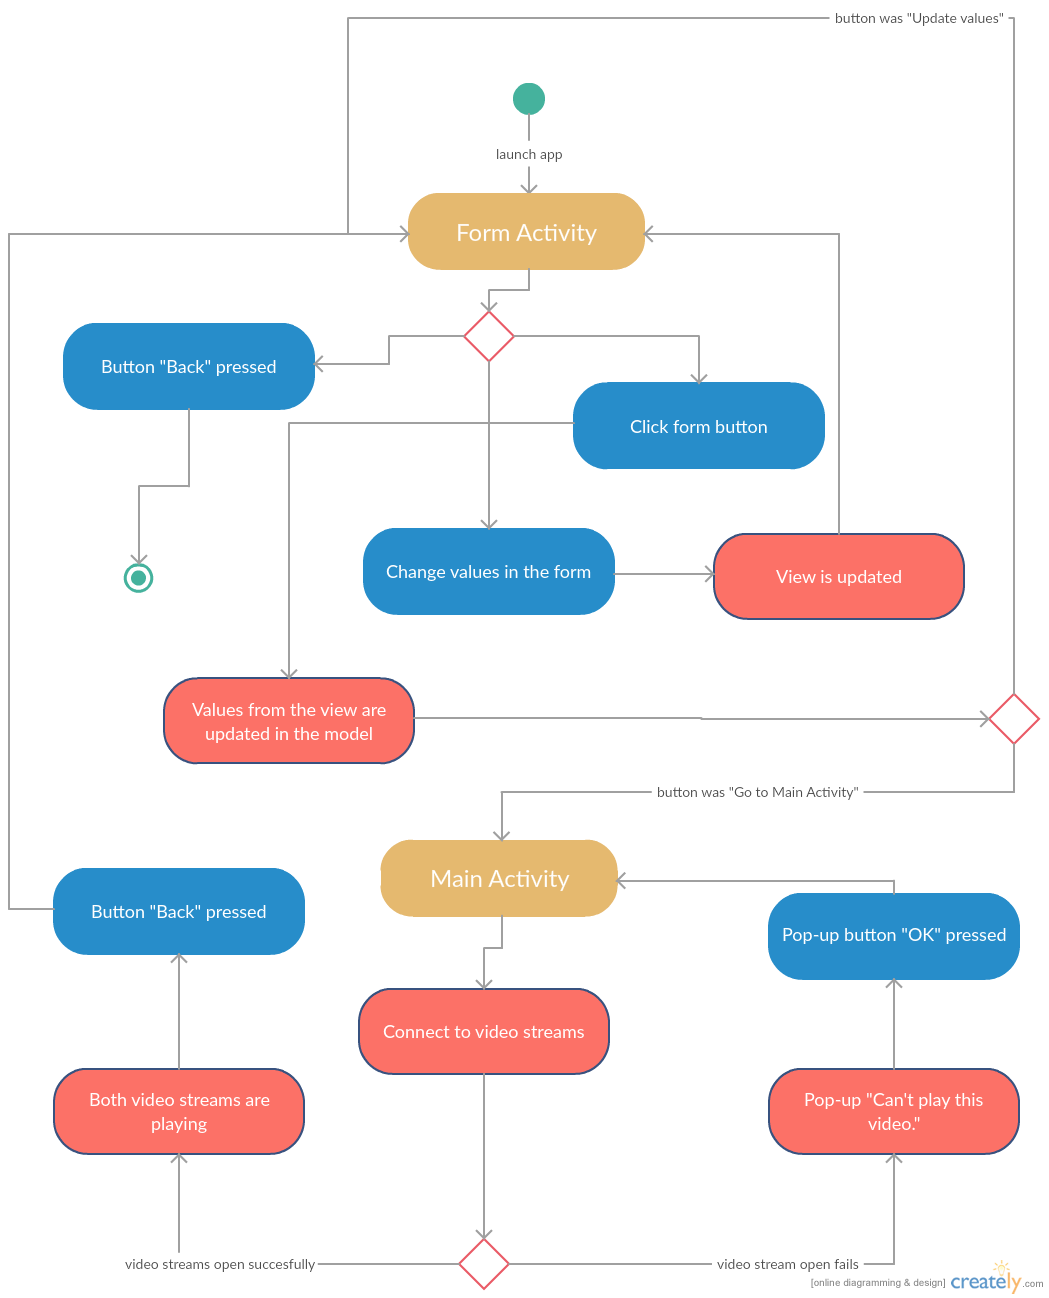
\includegraphics[width=7.00in]{images/diagrama_actividad.png}}
	}
	\caption{\textbf{Diagrama de actividad de la aplicaci�n para Android}. En ocre, las vistas de la aplicaci�n. En azul, las interacciones del usuario. En rojo, las respuestas del sistema.}
	\label{fig:diagrama_actividad_app}
\end{figure}

%\todo[inline]{Dise�o: \textbf{Diagrama de secuencia}}



\chapter{Implementaci�n}
\label{chap:implementacion}


\lsection{Cliente}
\subsection{Fundamentos de programaci�n para Android con Android Studio}
\todo[inline]{Implementaci�n: \currentname}
\textbf{Referencias a libro de Android de la biblioteca}
\begin{itemize}
\item Activity
\item Layout
\item Interfaces handler (?)
\end{itemize}
\subsection{Aplicaci�n}

Est� compuesta por 4 clases escritas en Java, de las cuales 2 extienden a la clase Android.Activity y las otras 2 son clases auxiliares. 

\subsubsection{Gestor de direcciones}

Esta clase implementa el patr�n de dise�o \textit{Singleton} (fragmento~\ref{fig:addressmanager_singleton}). Forma parte del modelo de la aplicaci�n y almacena las direcciones y puertos de los servidores. Permite leer y escribir estos datos (fragmento~\ref{fig:addressmanager_atributos}) independientemente de la actividad en la que se encuentre el usuario a trav�s de sus m�todos de acceso p�blicos (\textit{getters} y \textit{setters}).


\subsubsection{Transmisor de posici�n}

Esta sencilla clase auxiliar est� asociada a un socket UDP que se crea en el constructor de esta misma, asociado a su vez a un puerto y una direcci�n IP determinadas (fragmento~\ref{fig:positionsender_constructor}). Encapsula las operaciones b�sicas con sockets, haciendo m�s sencilla la comunicaci�n con el servidor de control a nivel de programaci�n (fragmento~\ref{fig:positionsender_send}).

\subsubsection{Formulario}

Esta actividad se muestra al iniciar la app. Al iniciarse, carga su layout a partir del fichero \textit{form.xml} y guarda la referencia a la instancia �nica del gestor de direcciones (fragmento~\ref{fig:formactivity_clase}). Las direcciones de sendos servidores multimedia con los streamings de v�deo han de ser indicadas mediante la URI completa, mientras que el servidor de control ha de indicarse introduciendo la direcci�n IP de la m�quina en la que se encuentra alojado el servidor y el puerto por separado. Los valores que se muestran en la figura~\ref{fig:captura_formulario} son los valores por defecto de estos \textit{textboxs} que coinciden con las direcciones en las que se despliegan los servidores en el entorno de trabajo para agilizar as� las pruebas.

En el archivo XML asociado a esta actividad, tambi�n se indica el nombre de los \textit{handlers} de los botones; es decir, la funci�n que se ejecutar� al clickar sobre cada uno de estos dos elementos. As� pues, esta clase debe implementarlos. Al presionar el bot�n \textit{Update values}, esta clase accede al valor de todos los \textit{textboxs} y los almacena en el gestor anteriormente explicado (fragmento~\ref{fig:formactivity_updatevalues}). Al presionar el segundo bot�n, se abandona esta actividad y se inicia la aplicaci�n principal, \textit{MainActivity} (fragmento~\ref{fig:formactivity_nextactivity}).


\begin{figure}[h]
	\centerline{
		\mbox{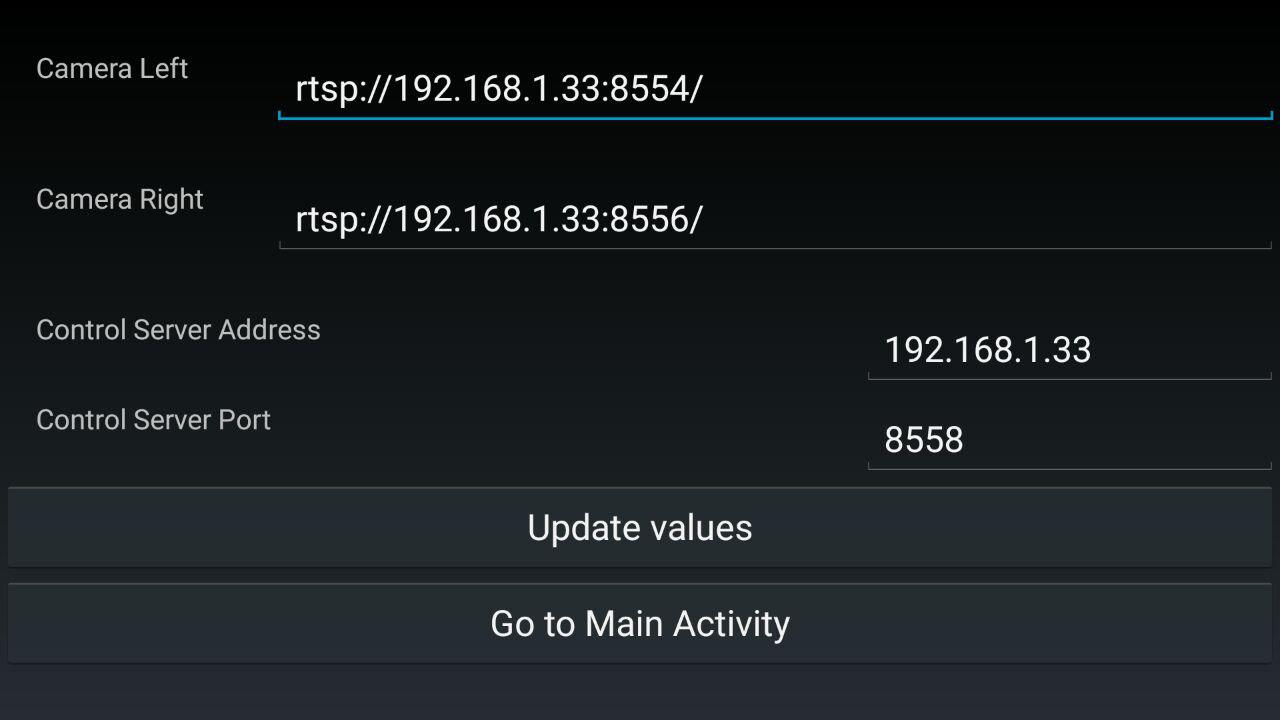
\includegraphics[width=4.00in]{images/captura_formulario.jpg}}
	}
	\caption{\textbf{Formulario de la aplicaci�n m�vil}. Permite al usuario modificar las direcciones de los tres servidores}
	\label{fig:captura_formulario}
\end{figure}


\subsubsection{Actividad principal}

Como en la actividad del formulario, al crearse se guarda la referencia al \textit{Singleton} y se carga el \textit{layout} a partir de su correspondiente archivo XML. En �ste se indica que habr� dos vistas, correspondientes a sendos \textit{streams} de v�deo, ocupando la pantalla completa mitad y mitad.

\begin{itemize}

\item Seguidamente, se crean dos reproductores de v�deo que se situar�n en estas dos vistas. En los constructores de estos objetos se pasan como par�metros las URI de los dos \textit{streams}, lo que har� que los v�deos se reproduzcan tan pronto como estos dos recursos est�n disponibles (fragmento~\ref{fig:mainactivity_videoviewinit}). 
\item Se obtienen las referencias a los sensores a trav�s del sistema operativo, mediante los cuales se calcular�n las rotaciones del dispositivo m�vil. Estos son el aceler�metro y la br�jula.
\item Se instancia un objeto de la clase Sender a partir de la IP y el puerto del servidor de control almacenados en el \textit{Singleton} (fragmento~\ref{fig:mainactivity_setupsensorposition})
\item Se crea el hilo que se encargue de enviar constantemente la posici�n, como se muestra en la figura~\ref{fig:coordenadas_polares}). A priori, la soluci�n m�s obvia es crear una clase que implemente la interfaz \textit{Runnable} y empezar un hilo mediante la clase \textit{Thread}. Tras este intento, el sistema operativo elimina este hilo porque, al parecer, consume mucha CPU, lo cual no permite a la actividad principal refrescar la interfaz gr�fica. Es decir, genera inanici�n. Como soluci�n y despu�s de investigar este contratiempo, encontr� la clase \textit{Handler} con su m�todo de instancia \textit{postdelayed}. Esencialmente, se inicializa este \textit{Hanlder} con un objeto que implemente \textit{Runnable} y postdelayed crea una alarma que se activar� despu�s de un determinado n�mero de milisegundos pasado como par�metro. Al activarse, se ejecute el m�todo \textit{run()} de este handler. Con esto, creamos un objeto \textit{Runnable} que ejecute una vez el cuerpo del bucle y finalmente vuelva a montar la alarma, como si se tratase de una recursi�n infinita (fragmento~\ref{fig:mainactivity_hilosender}).

\end{itemize}


\lsection{Servidores de v�deo}
\subsection{Streaming multimedia, c�decs y formatos de v�deo}
\todo[inline]{Implementaci�n: \currentname}
\subsection{Configuraci�n del servidor}

Para los servidores de v�deo, finalmente se ha utilizado el comando \textbf{cvlc}, herramienta de VLC para la terminal. �sta ofrece una inmensidad de servicios, entre los cuales no interesa la posibilidad de desplegar servidores multimedia. La configuraci�n de estos se indica junto con este comando en una cadena de caracteres que vendr� a definir el pipeline que se ejecutar� para dicho servidor. Un pipeline consta, en resumen, de estos elementos:

\begin{enumerate}
\item Entrada (\textit{Input Source})
\item Operaciones intermedias (\textit{Transcode})
\item Salida (\textit{Output Stream})
\end{enumerate}

Como entrada, se especifica la videoc�mara por su ruta dentro del sistema de ficheros y se abre en este caso con V4L2 que es una API de captura de v�deo y est� integrada en el kernel de linux.

Con esta fuente, se forma el v�deo en s�. El c�dec de v�deo elegido ha sido el \textbf{H264}. Este formato tiene decenas y decenas de variables y par�metros. Ya que el objetivo de este proyecto no era el de realizar una tarea de optimizaci�n tan intensa, se ha recurrrido a lo que se llaman \textit{presets}, que dan valor al conjunto de par�metros del c�dec para ofrecer una determinada calidad y rendimiento. Se ha configurado de forma que sea lo m�s r�pido posible y que tenga una menor latencia. Finalmente, se indica la resoluci�n de salida para que se corresponda justo lo que ocupar� en la aplicaci�n de m�vil (la mitad de la resoluci�n de la pantalla t�ctil) y tambi�n se indican los FPS).

Finalmente, se indica que la salida del pipeline ser� un servidor RSTP, en el cual se enviar�n los datos a trav�s de RTP y cuyos datos de sesi�n se guardar�n en un archivo SDP, que se encontar� en la direcci�n f�sica de la propia m�quina en la que se ejecute el script y en el puerto indicado.

El c�digo completo del script se encuentra en la figura ~\ref{fig:despliegue_servidores_video}
1

\lsection{Servidor de control}

\subsection{Servomotor y arduino}

\begin{figure}[H]
	\centerline{
		\mbox{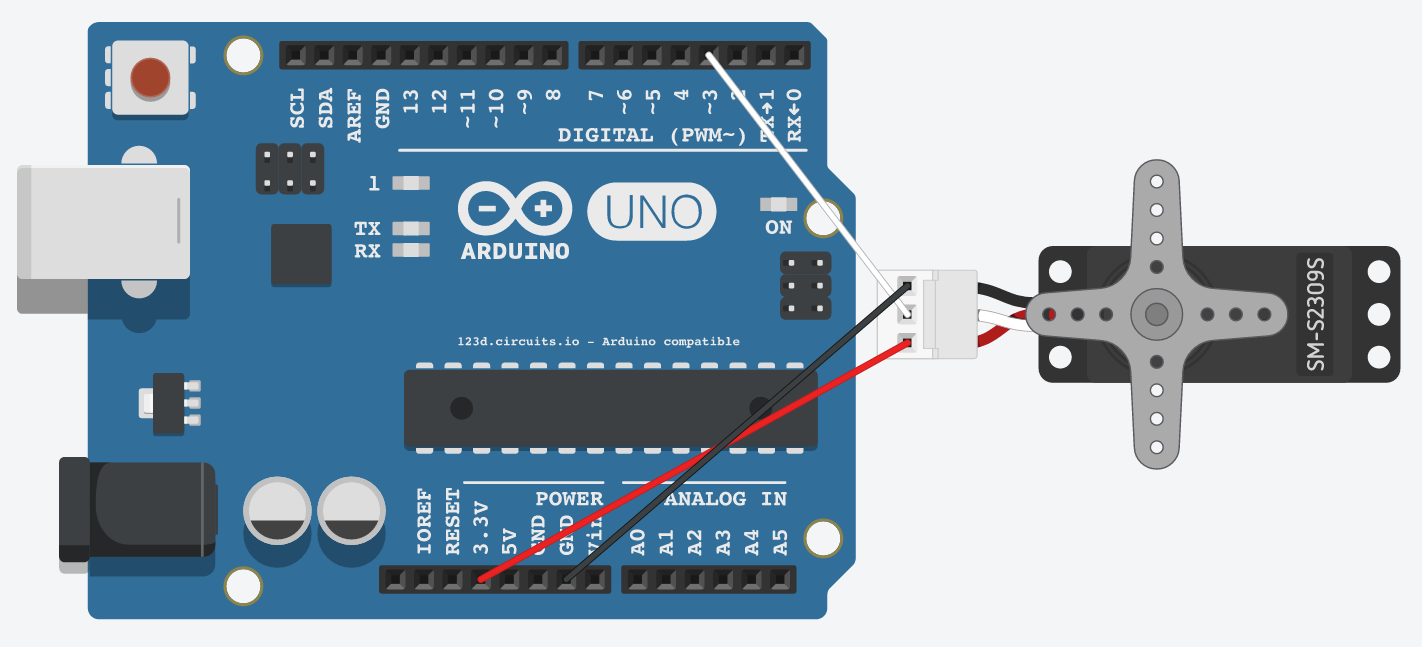
\includegraphics[width=4.00in]{images/circuito_arduino.png}}
	}
	\caption{\textbf{Circuito del Arduino controlando el servomotor}. El cable rojo va a VCC (3.3V) de la placa arduino, el cable negro a GND (tierra) y el cable blanco al PWM correspondiente. Variando el valor de la se�al anal�gica del PWM, conseguimos cambiar de sentido y de intensidad. }
	\label{fig:circuito_arduino}
\end{figure}


\subsection{Cliente/servidor UDP}
\todo[inline]{Implementaci�n: \currentname}
\subsection{Programaci�n del arduino}

Se ha utilizado la librer�a \cite{online:varspeedservo} para el control del servomotor.

\subsection{Programaci�n del servidor}
Para la implementaci�n de este servidor, se ha elegido Python 2.7 como lenguaje de programaci�n por los siguientes motivos:
\begin{itemize}
\item Es un lenguaje de muy alto nivel, potente, r�pido de programar y f�cil de depurar.
\item El m�dulo \textbf{socket} proporciona un manejo de bajo nivel de los propios sockets del sistema operativo que en realidad encapsula estas funciones propias de C/C++ en UNIX.
\item El m�dulo \textbf{serial} permite al programador acceder a cierto puerto serial para efectuar operaciones de lectura y escritura abstray�ndose del protocolo USB a bajo nivel.
\end{itemize}

\subsubsection{ServoController}
El constructor de esta clase intenta abrir el puerto serial donde ha de encontrarse conectado el Arduino y lanza una excepci�n cuando la apertura falla. Despu�s, simplemente se invoca al m�todo \textit{moveAngle()} que recibe un �ngulo como par�metro. Una instancia de esta clase siempre guarda internamente el �ltimo �ngulo recibido a trav�s de este m�todo (inicializ�ndolo en 0 grados) y el �ngulo que debe desplazarse se calcula mediante la diferencia con esta referencia. Es decir, el incremento del �ngulo es relativo al �ngulo inmediatamente anterior. Ya que el tipo de motor no es preciso a la hora de desplazar un �ngulo en concreto, se ha tomado la siguiente decisi�n de implementaci�n: se ha creado un diccionario en el cual las claves son un �ngulo en concreto, m�ltiplo de 45 y de -180 a 180. Los valores, son el valor anal�gico que hay que pasarle al arduino para que gire, aproximadamente, esa cantidad de grados. Por tanto, el valor que se enviar� a trav�s del puerto serial ser� el valor para la clave que m�s se aproxime a la diferencia entre el nuevo �ngulo y el �ngulo anterior (es decir, el incremento).

\subsubsection{UDP server}	
�ste es el programa que se encarga de realizar todas las tareas necesarias para desplegar el servidor de control en la m�quina en la que se ejecute.
\begin{itemize}
\item Al ejecutarse el proceso, se crea un socket UDP.
\item Se obtienen la direcci�n IP y el puerto que son pasados como argumentos al ejecutar el programa.
\item Se vincula el socket a esta direcci�n a trav�s del m�todo \textit{bind()}
\item Se intenta crear una instancia de \textit{ServoController}. Si hubiese un fallo, termina la aplicaci�n indicando el error que lo produjo.
\item Comienza el propio bucle del servidor:
	\begin{enumerate}
	\item Recibe de forma bloqueante del socket y muestra los datos recibidos.
	\item Parsea el mensaje para convertirlo de una cadena de caracteres a un n�mero en coma flotante.
	\item Llama al m�todo \textit{moveAngle()} de la instancia de \textit{ServoController} para realizar el movimiento angular
\end{enumerate}	
\end{itemize}



\chapter{Pruebas y resultados}
\label{chap:experimentos}

\lsection{Calidad de servicio}

Para medir la \textit{QoS}, se han hecho pruebas combinando distintos clientes, distintos servidores y distintos interfaces de red.
\todo[inline]{Pruebas: \currentname}
\subsection{Servidores}
A continuaci�n, se comentan las distintas implementaciones de los servidores multimedia que se han contemplado. Las siguientes herramientas listadas se ejecutan a trav�s de la terminal de Linux y los par�metros de los streams se especifican como argumentos de los correspondientes ejecutables:
\begin{itemize}
	\item \textbf{FFMpeg}
	\item \textbf{FFServer}
	\item \textbf{GStreamer}
	\item \textbf{CVLC}
\end{itemize}


\subsection{Clientes}

\begin{itemize}
	\item \textbf{FPlay}: se ejecuta a trav�s de la terminal y, a parte de mostrar el \textit{stream}, muestra por la terminal datos acerca de �ste.
	\item \textbf{VLC}: este famoso reproductor de multimedia tambi�n puede usarse para abrir contenido a trav�s de una URL. 
	\item \textbf{RTSP Player}: Es una \textit{app} para Android que se conecta a un v�deo RTSP a trav�s de su enlace.
	\item \textbf{Programa con JavaCV}: JavaCV utiliza wrappers para diversas librer�as de visi�n por computador. Este programa de elaboraci�n propia conecta con los servidores multimedia a trav�s de la URL y los muestra en dos ventanas, una al lado de la otra. La idea era poder portar este c�digo a la aplicaci�n de Android, utilizando el archivo .jar para ARM en vez del archivo para amd64. Al probarlo, surg�a un error inidentificable al abrir los \textit{streams} y, tras bastante esfuerzo intentando solventarlo sin resultado, hubo que buscar otra soluci�n.

\end{itemize}

\subsection{Interfaces}

\begin{itemize}
	\item \textbf{\textit{localhost}}: Pseud�nimo de la direcci�n IP 127.0.0.1, se usa para referirse a la propia m�quina. Para pruebas en las que el cliente y el servidor se encuentran ejecut�ndose en la misma m�quina. La p�rdida de paquetes es �nfima en este escenario.
	\item \textbf{Multicast Wi-Fi}: La �nica forma de desplegar el servidor RTSP utilizando un interfaz de red \textit{wireless}
	y que pudiese ser accedido desde otras m�quinas era utilizando una direcci�n IP multicast.
	\item \textbf{Unicast RJ-45}: Finalmente, el cableado a trav�s de un cable RJ-45 al router era la mejor opci�n (como era de esperar). Ofrece un MTU mayor, mayor ancho de banda y menos p�rdida de paquetes. Adem�s, permite desplegar el servidor en la direcci�n IP correspondiente a la interfaz de red (\textit{eth0}), lo cual hace que los servidores multimedia sean unicast, lo que quiere decir que s�lo se permite una conexi�n a la vez.
\end{itemize}

\subsection{Pruebas significativas}


\lsection{C�maras}
\label{sect:prueba_camaras}
\todo[inline]{Pruebas: \currentname}

\subsection{C�maras con objetivo ojo de pez}

Tambi�n conocidas como \textit{fisheye lens}, las lentes de estas c�maras proporcionan un �ngulo de visi�n superior al resto de tipos de lentes a cambio de una distorsi�n visual severa. Una vez montado todo el sistema, se ha probado a ejecutar la aplicaci�n con las gafas de realidad virtual y conect�ndose a los dos servidores de v�deos alimentados por fotogramas de estas c�maras. El cerebro parece no estar preparado para sentir la profundidad a partir de dos im�genes de este tipo y, a pesar de las prestaciones que podr�an haber ofrecido, las c�maras con objetivo de ojo de pez no han resultado id�neas para este proyecto.


\todo[inline]{\currentname: cambiar por imagen con fisheye}

\begin{figure}[H]
	\centerline{
		\mbox{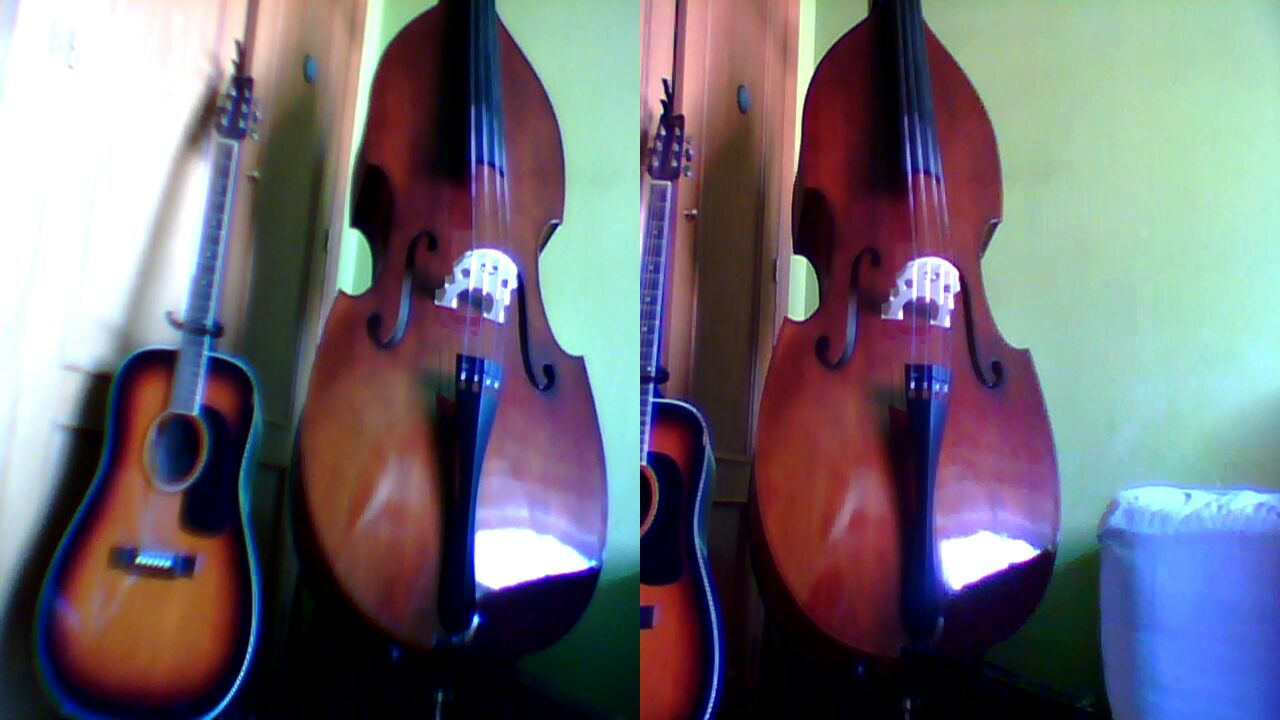
\includegraphics[width=4.00in]{images/captura_cliente_1.jpg}}
	}
	\caption{\textbf{Aplicaci�n funcionando con c�maras \textit{fish-eye} en los servidores de v�deo.} Esta imagen es una captura de pantalla del dispositivo Android desde el que se han hecho las pruebas.}
	\label{fig:captura_cliente_fisheye}
\end{figure}

\subsection{C�maras con lente normal}

Al final, unas webcam normales adquiridas en una tienda com�n de electr�nica han resultado las m�s adecuadas. Ya que no poseen esta curvatura tan pronunciada en las im�genes, es posible captar la profundidad ya que las equivalencias entre ambas im�genes son lineales. 

\begin{figure}[H]
	\centerline{
		\mbox{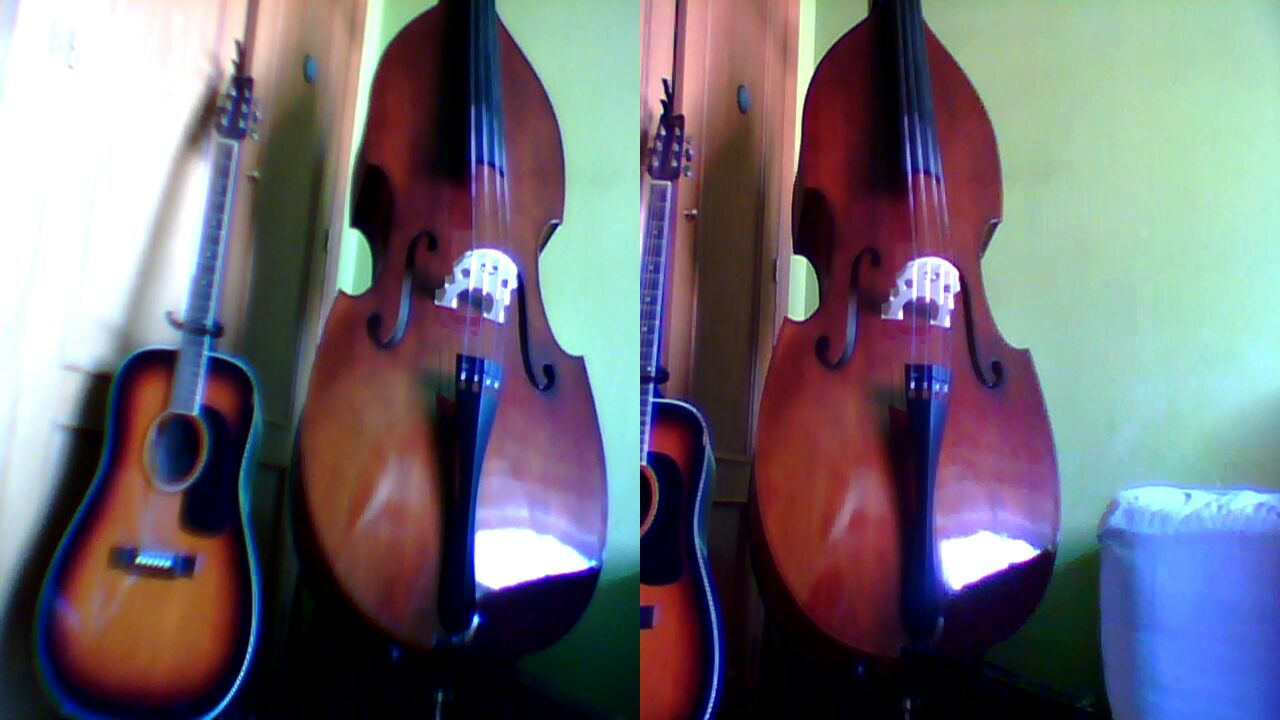
\includegraphics[width=4.00in]{images/captura_cliente_1.jpg}}
	}
	\caption{\textbf{Aplicaci�n funcionando.} Esta imagen es una captura de pantalla del dispositivo Android desde el que se han hecho las pruebas.}
	\label{fig:captura_cliente_1}
\end{figure}

\lsection{Servomotor}
\label{sect:prueba_servo}
%\todo[inline]{Pruebas: \currentname}

Los servomotores son capaces de girar en sentido horario o antihorario con mayor o menor velocidad angular. Esto se indica mediante una se�al anal�gica de entrada, la cual producimos en este caso mediante los PWM de la placa Arduino. En materia de c�digo, este valor se indica con un byte sin signo, es decir, un n�mero natural en el rango [0, 255], como se explica en \cite{online:pwm}. As� pues, despu�s de calibrar el motor con un destornillador se observando el comportamiento del servomotor para distintos valores anal�gicos. En el cuadro \ref{tabla:valores_servomotor} se encuentran estos resultados, que m�s tarde se usaron para la implementaci�n de la clase manda valores al Arduino a trav�s de un objeto \textit{Serial}.

\begin{table}[H]
	\centering
	\caption{}
	\label{tabla:valores_servomotor}
	\begin{tabular}{@{}ccc@{}}
		\toprule
		\multicolumn{1}{l}{Incremento del �ngulo ($^\circ$)} & \multicolumn{1}{l}{\begin{tabular}[c]{@{}l@{}}Valores para desplazar el \\ servomotor a la izquierda\end{tabular}} & \multicolumn{1}{l}{\begin{tabular}[c]{@{}l@{}}Valores para desplazar el \\ servomotor a la derecha\end{tabular}} \\ \midrule
		0                                             & 90                                                                                                                 & 90                                                                                                               \\
		45                                            & 79                                                                                                                 & 99                                                                                                               \\
		90                                            & 73                                                                                                                 & 104                                                                                                              \\
		135                                           & 73, 79                                                                                                             & 104, 99                                                                                                          \\
		180                                           & 60                                                                                                                 & 117                                                                                                             
	\end{tabular}
\end{table}

\lsection{Experimentos del sistema completo y resultados}
\todo[inline]{Pruebas: \currentname}




\chapter{Conclusiones y trabajo futuro}
\label{chap:conclusiones}


\lsection{Conclusiones}
%\todo[inline]{\currentname}

%Los objetivos principales de est<e proyecto se han visto realizados.

Personalmente y como logro propio, se ha llevado a cabo el desarrollo de un sistema distribuido heter�geneo, integrando tecnolog�as punteras y variadas como culmen de mis estudios en \carrera. 

El mundo de las redes multimedia y la transmisi�n de v�deo y audio tiene muchos detalles. A pesar de que no ha sido complejo integrar estas herramientas para desplegar un servidor de v�deo, las implementaciones de los protocolos a nivel de aplicaci�n de transmisi�n de multimedia (RTSP en este caso) son complejas a bajo nivel, as� como los c�decs, los formatos y todos sus par�metros, variables y metadatos, lo cual tendr�a que tomarse en cuenta en consiguientes fases de optimizaci�n.
		
Por otro lado y como se ha comentado previamente, la realidad virtual se encuentar en auge, motivo por el cual han surgido y surgen nuevas librer�as, herramientas, \textit{frameworks}, etc. orientados la creaci�n de programas y aplicaciones de VR. Al ser tan nuevas, todav�a necesitan madurar arreglando fallos y bugs, documentando mejor las APIs e implementando m�s funcionalidad necesaria y/o �til para el desarrollo de este tipo de software. A�n con esto, es el momento de desarrollar software de VR, ya sean aplicaciones para Cardboard o programas (videojuegos o software m�s comercial) para computadores de sobremesa para las nuevas plataformas que se est�n empezando comercializar actualmente.

JavaCV era una opci�n en el lado del cliente para manipular los \textit{streams} y los frames obtenidos de estos, pero por un fallo de implementaci�n del .jar para la arquitectura \textit{arm} se tuvo que renunciar a todo este potencial. A�n as�, OpenCV y sus versiones para \textit{x86} y \textit{amd64} ser�an una buen opci�n para un procesamiento previo al env�o u otro proyecto relacionado.

\newpage


\lsection{Trabajo futuro}
%\todo[inline]{\currentname}
Se ha llevado a cabo un prototipo con la funcionalidad b�sica del producto descrito en un principio. A continuaci�n se enumeran las distintas tareas que se podr�an llevar a cabo para obtener una versi�n mejorada de �ste.

\begin{itemize}

	\item {
		Tareas de optimizaci�n de la QoS, a saber:
		\begin{enumerate}
			\item Desarrollar una \textbf{vista} para Android (android.view.View) \textbf{espec�fica para streams RTSP}, que ofrezca mayores prestaciones tales como menor delay, mantener la sesi�n RTSP, sincronizaci�n de los dos flujos de v�deo, etc.
		\end{enumerate}
	}	
	\item Utilizar la API Google VR for Android \cite{link:googlevr}. Hasta hace unos meses, se llamaba Cardboard API. Actualmente tambi�n incluye soporte para DayDream VR \cite{link:daydream}, cuyo lanzamiento tendr� lugar en oto�o del 2016, y est� m�s documentada, con m�s ejemplos y m�s funcionalidad. Los v�deos se mostrar�an sobre una textura de OpenGL como en la figura~\ref{fig:cardboard_3d}
	\item Implementar la rotaci�n sobre los ejes X e Y (Pitch y Roll respectivamente, figura \ref{fig:coordenadas_polares}).
	\item \textbf{Utilizar motores paso a paso o \textit{steppers}} para mover la estructura sobre la que se encuentren las c�maras, ya que estos permiten girar un determinado arco con precisi�n, dependiendo de las especificaciones del componente.
	\item Modelar mediante un editor de 3D y posteriormente imprimir un exoesqueleto en el que puedan acomodarse las c�maras y que proteja los motores y circuitos de los golpes, el calor, etc.
	\item A�adir un stream m�s que se corresponda con el audio, grabado en el servidor a trav�s de un micr�fono cualquiera.
	\item Alojar la estructura con las c�maras y los motores sobre otro robot que proporcione movilidad, como un veh�culo teledirigido un dron.
\end{itemize}
\newpage \thispagestyle{empty} % P�gina vac�a 

\chapter*{Glosario de acr�nimos}
\addcontentsline{toc}{chapter}{Glosario de acr�nimos}

\begin{itemize}

\item{\textbf{VR}: \textit{Virtual Reality} (Realidad Virtual)}
\item{\textbf{HMD}: \textit{Head Mounted Display} (Gafas de Realidad Virtual)}
\item{\textbf{POC}: \textit{Proof Of Concept} (Prueba de concepto)}
\item{\textbf{UDP}: \textit{User Datagram Protocol}}
\item{\textbf{RTSP}: \textit{Real Time Streaming Protocol} (Protocolo de transmisi�n en tiempo real)}
\item{\textbf{SDP}: \textit{Session Description Protocol} (Protocolo de descripci�n de sesi�n)}
\item{\textbf{URI}: \textit{Uniform Resource Identifier} (Identificador de recursos uniforme)}
\item{\textbf{MVC}: \textit{Model View Controller} (Modelo Vista Controlador)}
\item{\textbf{IP}: \textit{Internet Protocol}}
\item{\textbf{V4L2}: \textit{Video4Linux v2}}
\item{\textbf{FPS}: \textit{Frames Per Second} (Fotogramas Por Segundo)}
\item{\textbf{PWM}: \textit{Pulse-Width Modulation}}
\item{\textbf{QoS}: \textit{Quality of Service (Calidad de servicio)}}
\item{\textbf{API}: \textit{Application Programming Interface}}
\item{\textbf{GPIO}: \textit{General Purpose Input Output}}
\item{\textbf{SDK}: \textit{Software Development Kit}}
\item{\textbf{IDE}: \textit{Integrated Development Environment}}


\end{itemize}

\newpage \thispagestyle{empty} % P�gina vac�a

\addcontentsline{toc}{chapter}{Bibliograf�a}    %Agregamos al �ndice el capitulo de bibliograf�a 

\bibliographystyle{unsrt}   %plain pero ordenado en orden de aparacicion en documento principal
\bibliography{bibliografia}

\appendix   %Indicamos que lo que viene a continuaci�n son ap�ndices

%\frontmatter %Para poner los anexos en numeros romanos

% Anexos

\chapter{Fragmentos de c�digo}
\label{Anexo:codigo}

A continuaci�n se muestran los fragmentos de c�digo m�s relevantes de cada uno de los componentes del sistema, con el fin de ayudar al lector a comprender las decisiones de implementaci�n.

\lsection{Cliente}

%\lstinputlisting[language=XML, firstline=1, lastline=106]{../01-CardboardApps/SurfaceViewCarboard/app/src/main/res/layout/form.xml}

\subsection{AddressManager.java}
%\todo[inline]{Anexo c�digo: \currentname}

\begin{figure}[H]
	\inputminted[firstline=7,lastline=12]{java}{\fpandroidclient/app/src/main/java/com/example/borch/surfaceviewcarboard/AddressManager.java}
	\caption{\textbf{Patr�n de dise�o \textit{Singleton}}. La �nica instancia de esta clase puede ser referenciada invocando al m�todo p�blico y est�tico \textit{getInstance()}}
	\label{fig:addressmanager_singleton}
\end{figure}

\begin{figure}[H]
	\inputminted[firstline=13,lastline=18]{java}{\fpandroidclient/app/src/main/java/com/example/borch/surfaceviewcarboard/AddressManager.java}
	\caption{\textbf{Atributos de la instancia}. Estos son los datos que se almacenan en esta clase. Sus correspondientes \textit{getters} y \textit{setters} son de acceso p�blico}
	\label{fig:addressmanager_atributos}
\end{figure}

\subsection{PositionSender.java}
%\todo[inline]{Anexo c�digo: \currentname}

\begin{figure}[H]
	\inputminted[firstline=17,lastline=24]{java}{\fpandroidclient/app/src/main/java/com/example/borch/surfaceviewcarboard/PositionSender.java}
	\caption{\textbf{Atributos de la clase}. }
	\label{fig:positionsender_atributos}
\end{figure}

\begin{figure}[H]
	\inputminted[firstline=27,lastline=33]{java}{\fpandroidclient/app/src/main/java/com/example/borch/surfaceviewcarboard/PositionSender.java}
	\caption{\textbf{M�todo constructor}. }
	\label{fig:positionsender_constructor}
\end{figure}

\begin{figure}[H]
	\inputminted[firstline=36,lastline=41]{java}{\fpandroidclient/app/src/main/java/com/example/borch/surfaceviewcarboard/PositionSender.java}
	\caption{\textbf{M�todo \textit{send()}}. Este m�todo se encarga de enviar un mensaje, en forma de una cadena de caracteres, a trav�s del socket UDP previamente inicializado en el constructor.}
	\label{fig:positionsender_send}
\end{figure}


\subsection{FormActivity.java}
%\todo[inline]{Anexo c�digo: \currentname}

\begin{figure}[H]
	\inputminted[firstline=12,lastline=22]{java}{\fpandroidclient/app/src/main/java/com/example/borch/surfaceviewcarboard/FormActivity.java}
	\caption{\textbf{Definici�n de la clase, AddressManager y \textit{onCreate()}}. }
	\label{fig:formactivity_clase}
\end{figure}

\begin{figure}[H]
	\inputminted[firstline=24,lastline=49]{java}{\fpandroidclient/app/src/main/java/com/example/borch/surfaceviewcarboard/FormActivity.java}
	\caption{\textbf{M�todo \textit{updateValues()}}. Controlador del bot�n \enquote{Update values}. Accede a los \textit{EditText} de la vista y los almacena en el modelo (AddressManager)}
	\label{fig:formactivity_updatevalues}
\end{figure}

\begin{figure}[H]
	\inputminted[firstline=52,lastline=57]{java}{\fpandroidclient/app/src/main/java/com/example/borch/surfaceviewcarboard/FormActivity.java}
	\caption{\textbf{M�todo \textit{nextActivity()}}. }
	\label{fig:formactivity_nextactivity}
\end{figure}


\newpage

\subsection{MainActivity.java}

\begin{figure}[h]
	\inputminted[firstline=91,lastline=110]{java}{\fpandroidclient/app/src/main/java/com/example/borch/surfaceviewcarboard/MainActivity.java}
	\caption{\textbf{Inicializaci�n de objeto VideoView}. El mismo proceso se realiza para myVideoViewRight y ambos comparten el mismo MediaController.}
	\label{fig:mainactivity_videoviewinit}
\end{figure}

\begin{figure}[h]
	\inputminted[firstline=133,lastline=142]{java}{\fpandroidclient/app/src/main/java/com/example/borch/surfaceviewcarboard/MainActivity.java}
	\caption{\textbf{Acceso a los sensores y creaci�n del objeto \textit{PositionSender}}: }
	\label{fig:mainactivity_setupsensorposition}
\end{figure}

\begin{figure}[h]
	\inputminted[firstline=161,lastline=174]{java}{\fpandroidclient/app/src/main/java/com/example/borch/surfaceviewcarboard/MainActivity.java}
	\caption{\textbf{Hilo de env�o} de la posici�n al servidor de control}
	\label{fig:mainactivity_hilosender}
\end{figure}

\begin{figure}[H]
	\inputminted[firstline=181,lastline=212]{java}{\fpandroidclient/app/src/main/java/com/example/borch/surfaceviewcarboard/MainActivity.java}
	\caption{\textbf{M�todo \textit{onSensorChanged()}}: Realiza el c�lculo de las coordenadas polares (figura~\ref{fig:coordenadas_polares}) cada vez que los sensores cambian de valor.}
	\label{fig:mainactivity_onsensorchanged}
\end{figure}

\begin{figure}[H]
	\inputminted[firstline=278,lastline=285]{java}{\fpandroidclient/app/src/main/java/com/example/borch/surfaceviewcarboard/MainActivity.java}
	\caption{\textbf{M�todo \textit{onBackPressed()}}: se ejecuta cuando se presiona el bot�n de los dispositivos Android con forma de tri�ngulo.}
	\label{fig:mainactivity_onbackpressed}
\end{figure}


\lsection{Servidores de v�deo}

\subsection{deploy.sh}
\begin{figure}[H]
	\inputminted[firstline=1,lastline=11]{bash}{\fpservidoresvideo/deploy.sh}
	\caption{\textbf{Script de despliegue} de los servidores multimedia.}
	\label{fig:despliegue_servidores_video}
\end{figure}	

\newpage

\lsection{Servidor de control}

\subsection{servo\_serial\_read.ino}
\begin{figure}[h]
	\inputminted[firstline=1,lastline=8]{cpp}{\fparduinocode/servo_serial_write/servo_serial_write.ino}
	\caption{\textbf{Cabecera del c�digo del Arduino}.}
	\label{fig:header_arduino}
\end{figure}	


\begin{figure}[H]
	\inputminted[firstline=9,lastline=27]{cpp}{\fparduinocode/servo_serial_write/servo_serial_write.ino}
	\caption{\textbf{Funci�n auxiliar \textit{myRead()}}. Lee caracter a caracter del puerto serial hasta encontrar el valor '\textbackslash n' y convierte la cadena de caracteres obtenida en un valor num�rico.}
	\label{fig:my_read_arduino}
\end{figure}	
%

\begin{figure}[H]
	\inputminted[firstline=27,lastline=34]{cpp}{\fparduinocode/servo_serial_write/servo_serial_write.ino}
	\caption{\textbf{Funci�n \textit{setup()} de Arduino}. Esta funci�n se ejecuta al arrancarse la placa.}
	\label{fig:setup_arduino}
\end{figure}	


\begin{figure}[H]
	\inputminted[firstline=36,lastline=43]{cpp}{\fparduinocode/servo_serial_write/servo_serial_write.ino}
	\caption{\textbf{Funci�n \textit{loop()} de Arduino}. Esta funci�n se ejecuta indefinidamente despu�s de ejecutarse \textit{setup()}.}
	\label{fig:loop_arduino}
\end{figure}	

\subsection{control\_servo.py}
%\todo[inline]{Anexo c�digo: \currentname}
\begin{figure}[H]
	\inputminted[firstline=28,lastline=34]{python}{\fpservidorcontrol/control_servo.py}
	\caption{\textbf{Definici�n de la clase y constructor de \textit{ServoControl}}. El �ngulo inicial es $\Psi_0 = 0^\circ$. El constructor crea un objeto \textit{Serial} en el puerto 9600 a partir de su ruta en el sistema operativo.}
	\label{fig:controlservo_clase}
\end{figure}

\begin{figure}[H]
	\inputminted[firstline=62,lastline=83]{python}{\fpservidorcontrol/control_servo.py}
	\caption{\textbf{Definici�n de la clase y constructor de \textit{ServoControl}}.}
	\label{fig:controlservo_moveangle}
\end{figure}

\subsection{udp\_server.py}

\begin{figure}[H]
	\inputminted[firstline=7,lastline=16]{python}{\fpservidorcontrol/udp_server.py}
	\caption{\textbf{Inicializaci�n de recursos del servidor de control}.}
	\label{fig:setup_udp_server}
\end{figure}

\begin{figure}[H]
	\inputminted[firstline=17,lastline=28]{python}{\fpservidorcontrol/udp_server.py}
	\caption{\textbf{Bucle del servidor de control}.}
	\label{fig:loop_udp_server}
\end{figure}


%\begin{listing}[ht]
%\inputminted{java}{../01-CardboardApps/SurfaceViewCarboard/app/src/main/java/com/example/borch/surfaceviewcarboard/MainActivity.java}
%\caption{Example from external file}
%\label{listing:3}
%\end{listing}

\newpage \thispagestyle{empty} % P�gina vac�a 

\chapter{Manual de usuario}
\label{Anexo:manual_usuario}

Manual de ayuda al usuario para utilizar el sistema.


\lsection{Repositorio}
\lsection{Uso}
\subsection{Despliegue de los servidores de v�deo}
\subsection{C�digo arduino}
\subsection{Despliegue de los servidores de v�deo}
\subsection{Despliegue de los servidores de v�deo}


\newpage \thispagestyle{empty} % P�gina vac�a 


%Hoja final en blanco
\newpage \thispagestyle{empty} % P�gina vac�a

\end{document}
